\documentclass{article}
\usepackage[utf8]{inputenc}
\usepackage[spanish]{babel}
\usepackage{graphicx}
\usepackage{float}
\usepackage{adjustbox}
\usepackage{subcaption}    
\usepackage{geometry}
\usepackage{tabulary}
\usepackage{tabto}
\usepackage{hyperref}

\geometry{
	a4paper,
	total={170mm,257mm},
	left=35mm,
	right=35mm,
	top=30mm,
	bottom=30mm,
}
 
\title{Memoria de Proyecto}
\author{Ingeniería web\\\\Grupo 13}
\date{Octubre 2021}
\setlength{\parindent}{2em}
\setlength{\parskip}{1em}
 
\begin{document}
 
\maketitle
 
\begin{figure}[H]
	 \captionsetup[subfigure]{justification=centering}
	  \begin{subfigure}[b]{0.49\textwidth}
		  \centering
			
\includegraphics[width=0.5\textwidth]{../images/Andoni.jpeg}
			\caption*{\textbf{Líder}: Salcedo Navarro, Andoni (785649)}
	  \end{subfigure}
	  \hfill
	  \begin{subfigure}[b]{0.49\textwidth}
		  \centering
		  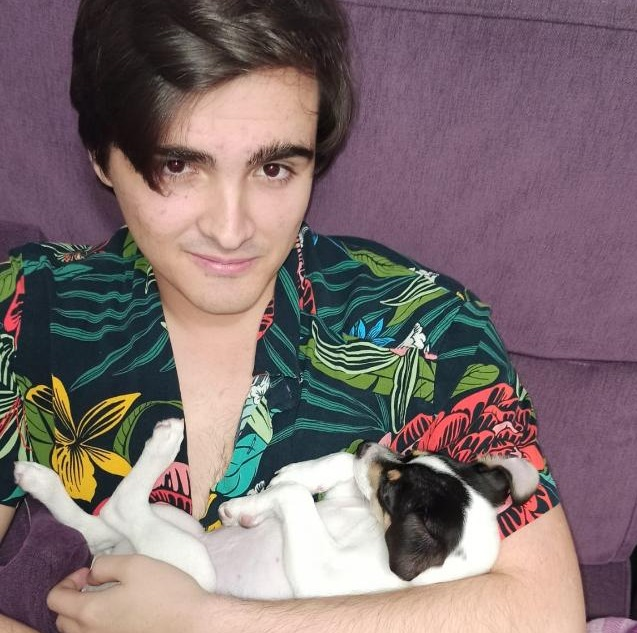
\includegraphics[width=0.5\textwidth]{../images/Tomas.jpeg}
		  \caption*{Pelayo Benedet, Tomás (779691)}
	  \end{subfigure}
	  \hfill
	  \begin{subfigure}[b]{0.49\textwidth}
		  \centering
		  
\includegraphics[width=0.5\textwidth]{../images/Ruben.jpeg}
		  \caption*{Subías Rodríguez, Rubén (759406)}
	  \end{subfigure}
	  \hfill
	  \begin{subfigure}[b]{0.49\textwidth}
		  \centering
		  
\includegraphics[width=0.5\textwidth]{../images/Isaac.jpeg}
		  \caption*{Velasco Calvo, Isaac (758986)}
	  \end{subfigure}
 
	 \end{figure}
 
\pagebreak

\section {Introducción y Objetivo}

Se ha creado una aplicación web, basada principalmente en SpringBoot\cite{springboot} y Kotlin\cite{kotlin}, buscando crear un servicio de acortación de URLs Web, añadiendo funcionalidades adicionales.

Los objetivos y funcionalidades principales que se querian añadir a esta aplicación son los siguientes:

\begin{itemize}
	 \item Los usuarios deben poder iniciar sesión y poder obtener información de aquellas
	 URLs que han acortado en el pasado.
	 \item La aplicación debe verificar que las URLs que se acorten sean alcanzables.
	 \item Un sistema de redirección para que el usuario pueda monetizar (La monetización está simulada con anuncios falsos)
\end{itemize}

\section {Organización}

Las tareas han podido ser divididas entre los miembros del equipo, con cada uno de ellos pudiendo hacer lo siguiente:

\begin{itemize}
	 \item \textbf{Andoni Salcendo}: Organización de proyecto y tareas, ????
	 \item \textbf{Tomás Pelayo}: ????
	 \item \textbf{Rubén Subías}: ????
	 \item \textbf{Isaac Velasco}: ????
\end{itemize}

\section {Funcionalidades y Tecnologías}

La mayoría de la interacción entre Backend y Frontend se realiza mediante una REST API creada con SpringBoot\cite{springboot}

\subsection{Gestión de URLs}

La gestión de URLs trata sobre el guardado de nuevas URLs acortadas y su recuperación, al igual que la gestión de códigos QR.

Para esto, se utiliza un Controlador de URLs (\texttt{controllers/UrlController.kt}), el cual usa una REST API para permitir todas las acciones que debe. Para acceder
a este controlador, se crea un punto de acceso con la URL \texttt{/api}.

La principal funcionalidad que permite este controlador es acortar URLs a partir del endpoint \texttt{/api/shorter}, el cual, al darle una URL completa, primero comprueba
que no exista ya en la base de datos. Si existe, devuelve la URL ya acortada, si no, comprueba si esta página es alcanzable con la función asincrónica, genera la versión acortada, la
guarda en la base de datos y la devuelve al usuario que realizo la petición. También genera el código QR si este ha sido pedido también.

También se puede recuperar aquellas URLs que han sido acortadas en el pasado por un usuario registrado en el endpoint \texttt{/api/user/urls} y el código QR de una URL acortada
si existe con \texttt{/api/qr}.

\subsection{Gestión de Usuarios}

TODO: Esto

\subsection{Gestión de Tiempo de Espera y Anuncios} \label{gestiontiempoespera}

En la pantalla de espera, donde el usuario debe esperar 10 segundos antes de recibir la URL des-acortada, se utiliza un WebSocket para, a la vez, forzar al usuario a esperar el tiempo
de espera deseado y obtener la URL real de una URL acortada.

Para esto configuramos un WebSocket de Springboot en \texttt{UrlShorterApplication.kt} y en \texttt{controllers/WSController.kt}. En el primer archivo, se realiza la configuración
básica del websocket con la clase \texttt{WSConfig}, como el endpoint donde se accede (\texttt{/wstimer}) e indicar a websocket que utilize cierta clase como controlador del WebSocket.
Esta clase es el controlador \texttt{controllers/WSController.kt} la cual gestiona que debe de hacer el WebSocket cuando recibe una petición desde un cliente, en este caso, esperar
10 segundos y devolver la URL real que ha pedido el usuario.

También en la pantalla de espera, se muestran anuncios elejidos de forma aleatoria por el backend. Esto se realiza con una controlador REST API en \texttt{controllers/AdController.kt},
el cual responde a aquellas peticiones HTTP al endpoint \texttt{/ad/obtain} con dos URLs a imagenes de anuncios falsos elejidos de una lista estática en el backend.

\subsection{Asincronía}

\subsection{Frontend}

React\cite{React} es una librería permite crear interfaces gráficas en páginas web.

Esta aplicación utiliza esta en su Frontend, donde la página se divide en diversas categorias/pantallas:

\begin{itemize}
	\item Página de Inicio (\texttt{UrlPage.jsx}): Esta pantalla es la que un nuevo usuario ve cuando se introduce por primera vez a la página web. Aquí se puede pedir recortar URLs, 
	generar QRs, Iniciar Sesión y Registrarse.
	\item Página de Inicio para Usuarios Registrados (\texttt{UrlUserPage.jsx}): Parecia a la pantalla anterior, pero con funcionalidades solo disponibles a usuarios registrados, como
	poder ver las URLs acortadas por este en el pasado y desconectarse de la aplicación.
	\item Página de Inicio de Sesión (\texttt{SingIn.jsx}): Usada para iniciar sesión en la aplicación web.
	\item Página de Registro (\texttt{SignUp.jsx}): Usada para registrarse en la aplicación web.
	\item Página de Espera (\texttt{WaitPage.jsx}): La página de espera que aparece cuando se intenta utilizar una URL acortada. Aquí, el usuario tendra que esperar 10 segundos para
	poder continuar a la URL deseada. Para poder esperar estos 10 segundos, se utiliza el WebSocket descrito en el apartado \ref{gestiontiempoespera}. También se muestran una serie de
	anuncios falsos, escojidos aleatoriamente de una colección por el backend, y se muestran al usuario.
\end{itemize}

Para poder comunicarse con el backend, exceptuando el uso de WebSockets para el tiempo de espera, se utiliza la libreria Axios\cite{Axios} para poder realizar peticiones HTTP.

\section{Pruebas}\newpage

\begin{thebibliography}{9}
	\bibitem{kotlin}
	Kotlin Programming Language - \url{https://kotlinlang.org/}
	\bibitem{springboot}
	SpringBoot - \url{https://spring.io/projects/spring-boot}
	\bibitem{springwebsocket}
	SpringBoot's Websockets - \url{https://spring.io/guides/gs/messaging-stomp-websocket/}
	\bibitem{React}
	React - \url{https://reactjs.org}
	\bibitem{Axios}
	Axios Documentation - \url{https://axios-http.com/docs/intro}
\end{thebibliography}
 
\end{document}
 
